Pour pouvoir faire fonctionner votre Raspberry Pi, vous avez besoin d'un système d'exploitation. Le système d'exploitation recommandé par la Raspberry Pi Foundation est Raspbian. Pour vous épargner la douleur de l'installation, nous l'avons déjà faite pour vous ;-) Vous pouvez donc dès à présent profiter du Raspberry.

Néanmoins, si un jour vous souhaitez utiliser votre propre Raspberry, il vous faudra passer par la case installation. Le reste de cette section vous explique comment procéder.

Installons donc le système d'exploitation. Il faut d'abord savoir qu'il n'y en a pas qu'un seul : le Raspberry Pi est pensé pour être un appareil multi-usages, il y a donc plusieurs systèmes d'exploitation! On peut y installer un système bureautique classique, semblable à Windows ou macOS, ou bien en faire une box multimédia qu'on connecte à la télévision. D'autres distributions sont dédiées à l'Internet des objets, c'est-à-dire les objets connectés.

Pour cette introduction, on va installer le système d'exploitation le plus connu, et le plus utilisé : Raspbian. Concrètement, il s'agit d'un système basé sur Linux, appelé Debian, mais optimisé pour fonctionner sur un Raspberry Pi.

Commencez par télécharger l'\textbf{image disque} de Raspbian sur \url{https://www.raspberrypi.org/downloads/raspbian/}. C'est un fichier assez lourd, il pèse en effet quelques gigaoctets.

Une fois l'image disque téléchargée, il faut la graver sur la carte micro-SD. Il y a plusieurs moyens d'y parvenir. Pour les plus téméraires, on peut utiliser la console; des instructions sont disponibles sur le site officiel\footnote{Voir en bas de cette page : \url{https://www.raspberrypi.org/documentation/installation/installing-images/README.md}}. Cependant, ce sont des manipulations avancées. On se contentera d'utiliser le programme Etcher, disponible sur Windows, macOS, et Linux en général, et très facile d'utilisation. Vous pouvez le télécharger ici : \url{https://etcher.io}.

\begin{figure}[h!]
\begin{center}
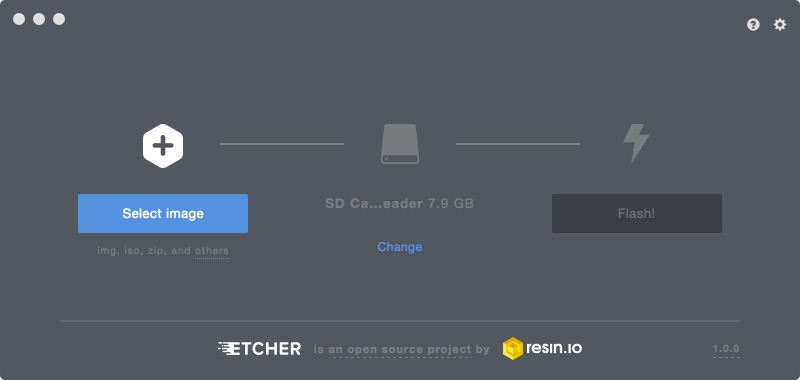
\includegraphics[width=10cm]{etcher.jpg}
\end{center}
\caption{L'interface très simple de Etcher}
\label{etcher}
\end{figure}

Sur la figure \ref{etcher}, on peut voir la seule et unique fenêtre de Etcher. En cliquant sur le bouton de gauche, vous pouvez sélectionner l'image disque. Elle devrait être au format \texttt{.img}. Si ce n'est pas le cas (\texttt{.zip} par exemple), il faudra la \textit{dézipper}. \textit{7zip} sur Windows et \textit{The Unarchiver} sur macOS permmettent de le faire.

Avec le bouton du milieu, sélectionner votre carte micro-SD dans l'explorateur de fichiers. Enfin, appuyez sur le bouton de droite "Flash!" pour graver l'image disque. L'opération prend environ 10 minutes.

Un fois ceci fait, profitez-en déjà pour activer une fonctionnalité dont nous aurons besoin : le SSH, qui permet d'accéder au Raspberry Pi à distance. Seulement, il y a quelques mois, une attaque informatique de grande envergure a utilisé des milliers d'appareils connectés pour affaiblir les serveurs des plus grands sites Internet. Suite à ça, l'entreprise qui produit les Raspberry Pi a décidé de désactiver le SSH par défaut, par mesure de sécurité.

Ce n'est pas grave, on peut le réactiver! Il suffit de créer n'importe quel fichier (avec un éditeur de texte par exemple), peu importe son contenu, de le nommer \texttt{ssh} (sans extension), et de l'ajouter à la \textbf{racine} de la carte micro-SD. La racine constitue le tout premier niveau d'un disque; c'est simplement la première chose qu'on voit quand on ouvre le disque dans un explorateur de fichiers.

Lors du premier démarrage, le Raspberry Pi détectera la présence du fichier, activera le SSH, et puis supprimera le fichier, tout simplement.